\documentclass[a4paper,11pt]{article}
\usepackage{fullpage}
\usepackage[utf8]{inputenc}
\usepackage{braket}
\usepackage{graphicx}
\usepackage[margin=.9in]{geometry}
\usepackage{makecell}
\usepackage{amsmath}
\usepackage{amssymb}
% \usepackage{subfigure}
%\usepackage{minipage}
\usepackage{bm}
\usepackage{multirow}
\usepackage{lipsum}
\usepackage{caption}
\usepackage{subcaption}
\usepackage{multicol}
\usepackage{float}
\usepackage[version=4]{mhchem}
\usepackage[colorlinks=true, linkcolor=blue, urlcolor=blue, citecolor=blue, anchorcolor=blue]{hyperref}
\usepackage[toc,page]{appendix}


% Keywords command
\providecommand{\keywords}[1]
{
  \small	
  \textbf{\textit{Keywords---}} #1
}

\author{Apoorav Singh Deo}
\author{}

\title{Sub-surface Object detection using Gravity Gradient Tensor derived from a vertical gravity component.}

\begin{document}

    
\maketitle

\noindent \abstract{Sub-surface Modelling is widely used in sectors such as Civil Engineering, Mineral Exploration, geoscience, etc. Mapping the subsurface shows the object lying below the earth without disturbing the test area. Therefore, such techniques can probe items below the surface without disturbing their chemical or physical signature. Using a precise gravimeter, the subsurface can be imaged with great precision. But a simple gravity ($g_z$) component is not enough. The gravity gradient tensor provides a good ground to describe subsurface anomalies better. Hence, using $g_z$ to obtain tensor components of gravity gradient tensor (GGT) can help us to utilize the formulation based on the GGT.}

\noindent \textbf{Keywords:} {Gravity anomaly; 
 Fourier transform; Gravity gradient tensor (GGT); Inverse Modelling;}


\section{Introduction}

\noindent Data from simple gravimeters that make acceleration measurements in the z-direction are readily available. That makes working with vertical gravity ($g_z$) data easy. The information and formulation available for the vertical gravity anomaly don't reveal much about the shallower part of the earth. Since applying gravity gradiometry may be expensive and challenging, the acceleration due to gravity ($g_z$) decays slowly compared to the gravity gradient tensor (GGT); therefore, the gravity gradient tensor is more sensitive to shallower anomalies \cite{Paoletti2016}. The gravity gradient method is frequently employed in interpretation for isolating gravity anomalies \cite{murphy2009exploring}. Further, the data for GGT is unavailable, and surveys using gradiometers are not widely done. This makes data availability scarce.\medskip

\noindent This paper discusses the possibility of using GGT calculated from the vertical component of the gravity field $g_{z}$ using the Fourier model \cite{mickus2001complete}, which can be used to estimate the mass of the anomaly and get a rough estimate of the center of mass $(x, y)$ of the detected object using inverse model \cite{tang2017analytical}. The gravity gradient tensor (GGT) is the second-order derivative of the gravitational potential or rate of change of the gravitational acceleration vector to the given displacement axis. When compared to the gravity acceleration in the z-axis ($g_{z}$) \cite{bouman2016satellite}, GGT has nine components with a significantly higher resolution in inverting the spatial position of target anomaly bodies, which means it will provide more information to help better understand the interior structure of the earth\cite{peters2001high}.\medskip

\noindent Now, the obtained GGT can be used to compute the mass of the anomaly as mentioned in the paper \cite{tang2017analytical}. Using the mass distribution obtained earlier, the body's center of mass can be estimated. The model was tested by varying factors such as density and depth, whose results are shown in the paper's result section. 

\section{Work Flow}
In this paper, the scheme that was followed is mentioned as follows.

\begin{enumerate}
    \item To test the scheme, test data was generated using the prism model \cite{plouff1975derivation} \cite{plouff1976gravity}. A simple vertical gravity component ($g_z\ \hat{k}$) is worked out.
    \item The Fourier model processes the test data obtained \cite{mickus2001complete}, gravity gradient tensor (GGT) is computed as well as the other two components of gravity acceleration are also computed ($g_x\ \hat{i}$, $g_y\ \hat{j}$).         

    \item Now, using the processed data and inverse model \cite{tang2017analytical}, we can estimate the mass of an unknown or known object and a rough estimate of the center of mass in the (x, y) plane.
    
\end{enumerate}

\begin{figure*}
    \centering
    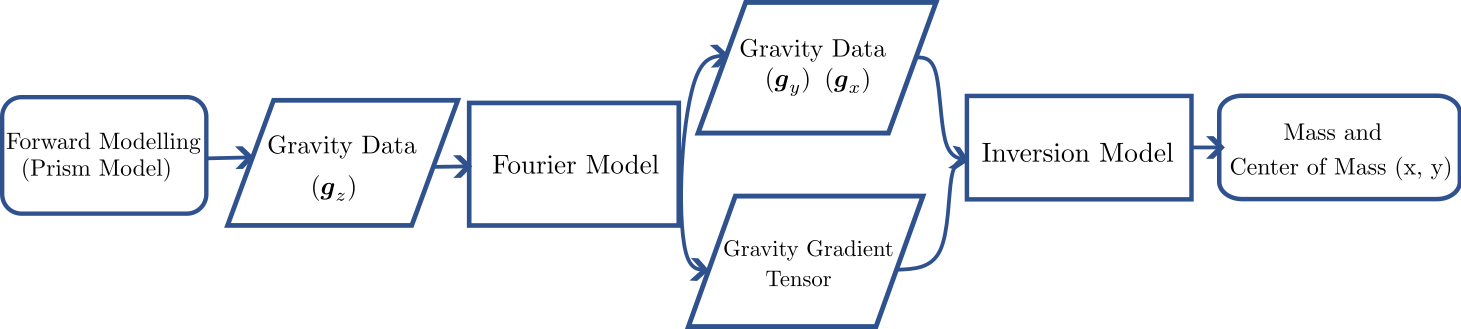
\includegraphics[scale=2.25]{images/flow.png}
    \caption{Work Flow}
\end{figure*}

\section{Numerical Results}

\subsection{Forward Modelling}

\noindent Gravity data is generally used to investigate subsurface geology based on mass distribution. To obtain the gravity attraction components and components of the spatial derivative of gravitational attraction, many models are used as a forward model; among them, the Right rectangular prisms model is used often. Many researchers have worked on this model to improve this. 

\noindent To provide the model with the test data. Gravity anomaly is being calculated using the model mentioned. Although this model can compute all the components needed for the calculation, only the $g_z$ is computed. Therefore, an attempt is made to simulate the data retrieved from a one-dimensional gravimeter. 

\subsubsection{Right rectangular prisms model} 


\begin{figure}[ht]
     \centering
     \begin{subfigure}[b]{0.4\textwidth}
         \centering
         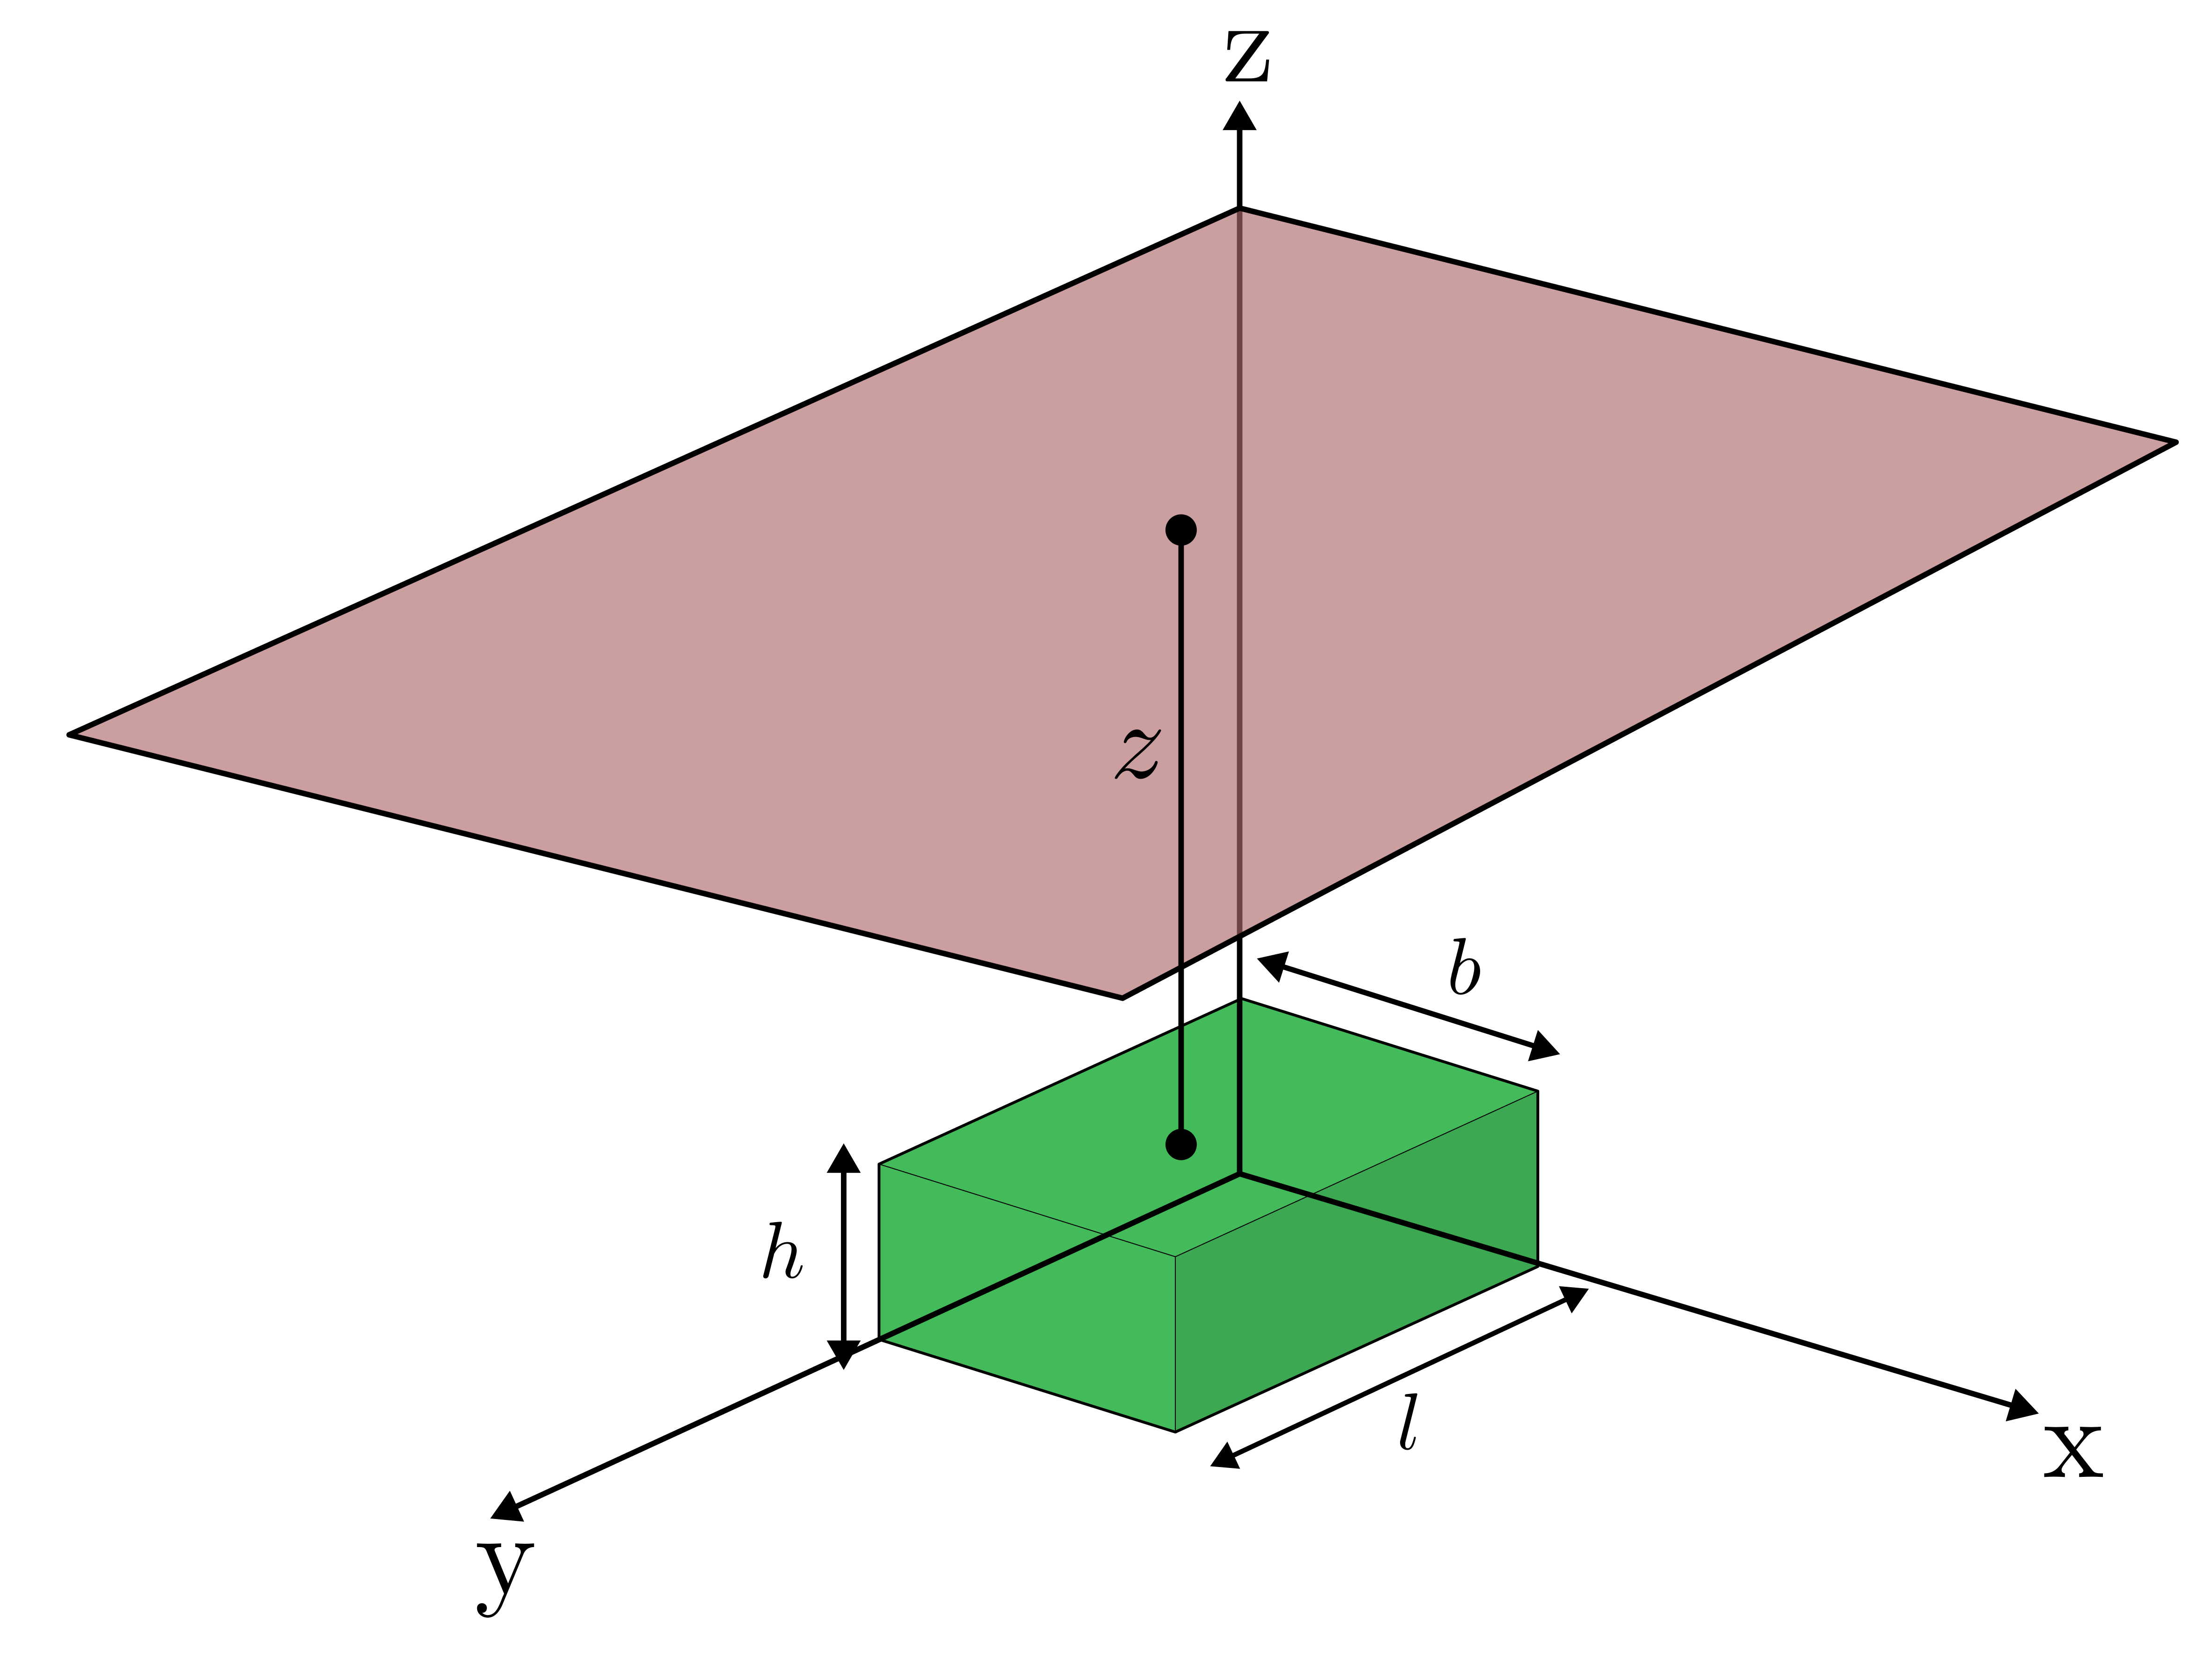
\includegraphics[scale = 0.4]{images/anomaly_illustraion.png}
         \caption{Test Mass under consideration.}
         \label{fig:gz1}
     \end{subfigure}
     \hfill
     \begin{subfigure}[b]{0.4\textwidth}
         \centering
          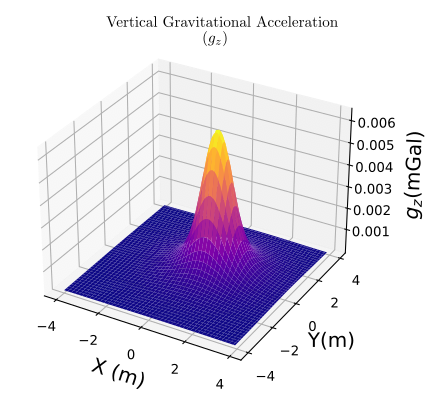
\includegraphics[scale = 3.6]{plots/gravity_ana.png}
         \caption{$g_{z}$ for the anomaly.}
         \label{fig:gz2}
     \end{subfigure}
        \caption{Model for Gravity Anomaly }
        \label{fig:gz}
\end{figure}


We have taken the \textbf{right rectangular prisms model} as a forward model to calculate the vertical gravitational acceleration. The rectangular prisms model method is a simple way of estimating the volume of a mass. Every prism may be assumed to have a static density if it is small enough. Using the superposition principle, we can obtain the gravity anomaly at any point of the body that could be approximated by adding the effects of all the prisms.
The equation of vertical gravitational acceleration of the right rectangular prism body is \cite{li1998three}


\begin{equation} \label{1}
    g_{z} = -G \rho\,\sum_{i=1}^{2}\,\sum_{j=1}^{2}\,\sum_{k=1}^{2}\,\mu_{ijk}[x_{i}\ln{(y_{j}+r_{ijk})}+y_{j}\ln{(x_{i}+r_{ijk})} \\
    - z_{k}\arctan(\frac{x_{i}\,y_{j}}{z_{k}\,r_{ijk}})]
\end{equation}

\noindent In our model, we assumed a rectangular prismatic body has a uniform density of $1400 kg/m^3$ that placed a $(z=1m)$ distance from the observing plane to the $x-y$ plane. The height $(h=0.5m)$ of the body along $z-$direction, length$(l=1.2m)$ along $y-$direction and breadth $(b=0.9m)$ in the $x-$direction as shown in Figure (\ref{fig:gz1}). We computationally define the vertical component of gravitational acceleration $(g_{z})$ in $mGal$ unit Using equation(\ref{1}) for this rectangular prismatic body shown in Figure (\ref{fig:gz2}). This component computed the other two horizontal gravitational acceleration components and full gravity gradient tensor for this prismatic body described in the next section. 

\subsection{Calculating Gravity Gradient Tensor}
The gravity gradient tensor is a symmetric, traceless matrix. Mathematically, it represents the rate of changes in gravitational acceleration with respect to the position in three dimensions. The fundamental gravity gradient tensor is important in gravity field modeling and analysis. It has numerous significance in various areas, including geodesy, geophysics space missions, and satellite navigation. The gravity gradient tensor is used in gravity field modeling, which uses gravitational data to determine the mass distribution inside the earth's surface.

\begin{figure}[ht]
    \centering
    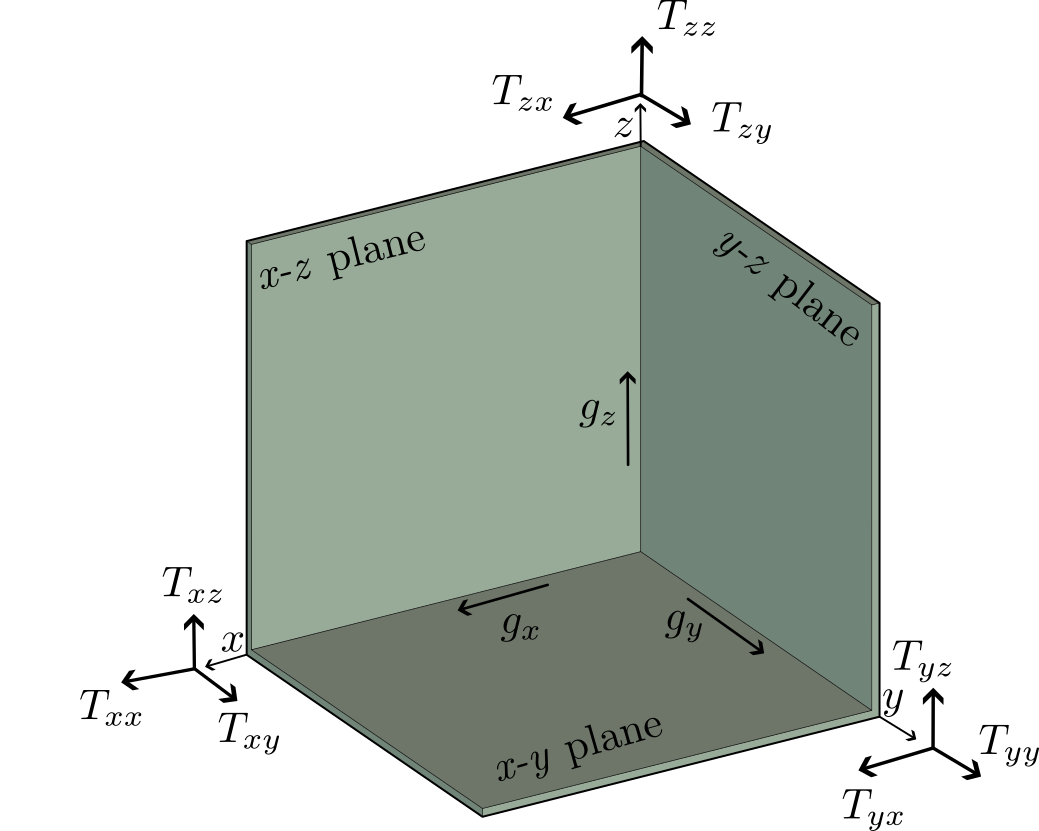
\includegraphics[scale=2.5]{images/coordinate_system.png}
    \caption{Schematic diagram of gravity gradient tensor components }
\end{figure}

\noindent Typical gravity information demonstrates the strength of the earth's gravity field but is less sensitive to object edges and missing the directional information. Gravity gradients directly recover acute signals across the borders of structures and are strongly connected to the causative entities like edges, corners, and center of mass, producing complex layouts of the anomalies. The Six gravity gradient components make a strong tool for outlining the body's contour. The vertical tensor component of $T_{zz}$ accounts for the boundary information specifically linked to the geological body and estimates the maximum depth. The $T_{xx}$ component indicates a feature of the $y-z$plane of the object. The $T_{yy}$ horizontal gradient component is along the edges of the $x-z$ plane of the object. In the $y-z$ plane, $T_{xy}$ component locates the body's center point and provides information on corners of the body along the $y-$ direction. $T_{zx}$ locates along the $x-$ direction in $x-y$ plane. $T_{yz}$ represents along the $z-$ direction in $x-z$ plane.\cite{menoret2018gravity} 

\noindent So, In this section, nine gravity gradient tensor (GGT) components are calculated using the Fourier model. Using this model, not only gravity gradient tensor is computed, but acceleration $(g_{x}, g_{y})$ is obtained too \cite{mickus2001complete}. Therefore, data processed through this model provides us with the recipe to continue with our inverse model. Hence, making computation via formulas only available for gravity gradient tensor\medskip

\noindent Three gravity components obtained are continuous, differentiable in nature,

\begin{equation} \label{2}
    \Vec{\textbf{g}}(x,y,z)= g_{x}(x,y,z)\hat{i} + g_{y}(x,y,z)\hat{j} + g_{z}(x,y,z)\hat{k}
\end{equation}

Here the vertical component$(g_{z})$ is measured at a distance $z=1m$ from the $x-y$ plane. Since $\Vec{g}$ is a conservative field, it satisfied the relation of equation (\ref{3}) and (\ref{4})

\begin{equation} \label{3}
     \vec{\nabla}\cdot \vec{g} =0
\end{equation}

\begin{equation}\label{4}
\vec{\nabla}\times \vec{g} = 0
\end{equation}

From The Fourier transform of Laplace's equation in $k_{x}-k_{y}$ plane 

\cite{blakely1996potential}, we have write \begin{equation}\label{5}
    \Vec{\textbf{k}}(x,y,z)= k_x(x,y,z)\hat{i} + k_y(x,y,z)\hat{j} + k_z(x,y,z)\hat{k}
\end{equation}

\noindent In $2-D$ plane, ${|\textbf{k}|}=-ik_{z} =\sqrt{k_x^2+k_y^2}$ \medskip
where $k_x, k_y,k_z $ are the reciprocal of spatial distances, wave vectors along different three axes $x-,y-,z-$ direction. The Fourier transform pairs were established using equation(\ref{4}).

\begin{subequations} \label{eq:6} 
\begin{align} 
\frac{\partial g_{z}}{\partial y}=\frac{\partial g_{y}}{\partial z} \leftrightarrow (-ik_{y})G_{z} = |\textbf{k}| G_{y} \label{sub-eq-1:6}\\
\frac{\partial g_{x}}{\partial z}=\frac{\partial g_{z}}{\partial x} \leftrightarrow |\textbf{k}|G_{x}  =(-ik_{x}) G_{z} \label{sub-eq-2:6}\\
\frac{\partial g_{y}}{\partial x}=\frac{\partial g_x}{\partial y}\leftrightarrow  -ik_{x}G_{y} =-ik_{y}G_{x} \label{sub-eq-3:6} 
\end{align}
\end{subequations}

%%%%%%%%%%%
\noindent Such that $ g_{x},\ g_{y}\, g_{z}\ $ are the perpendicular elements of $\Vec{\textbf{g}}$ and $G_{x}(k_x,k_y), G_{y}(k_{x},k_{y}), G_{z}(k_x,k_y)$ are the two dimensional Fourier transform of $g_{x}, g_{y}, g_{z}$. \medskip

Equation(\ref{9}) represents the Inverse Fourier Transform (FFT) of multiplication of the matrix of wave vector with Fourier transform of gravity along $z-$ direction. Using the equation(\ref{7}), we computed two other horizontal components of gravitational acceleration from the Fourier transform values of the vertical gravity component$(G_{z})$.
 
\begin{equation}\label{7}
g_{i} \leftrightarrow G_{i}= \frac{(-ik_{i})}{|\textbf{k}|}G_{z}\textbf{(k)}
\end{equation}

\noindent Where $i= x,y$, 
\begin{figure}[ht]
    \centering
    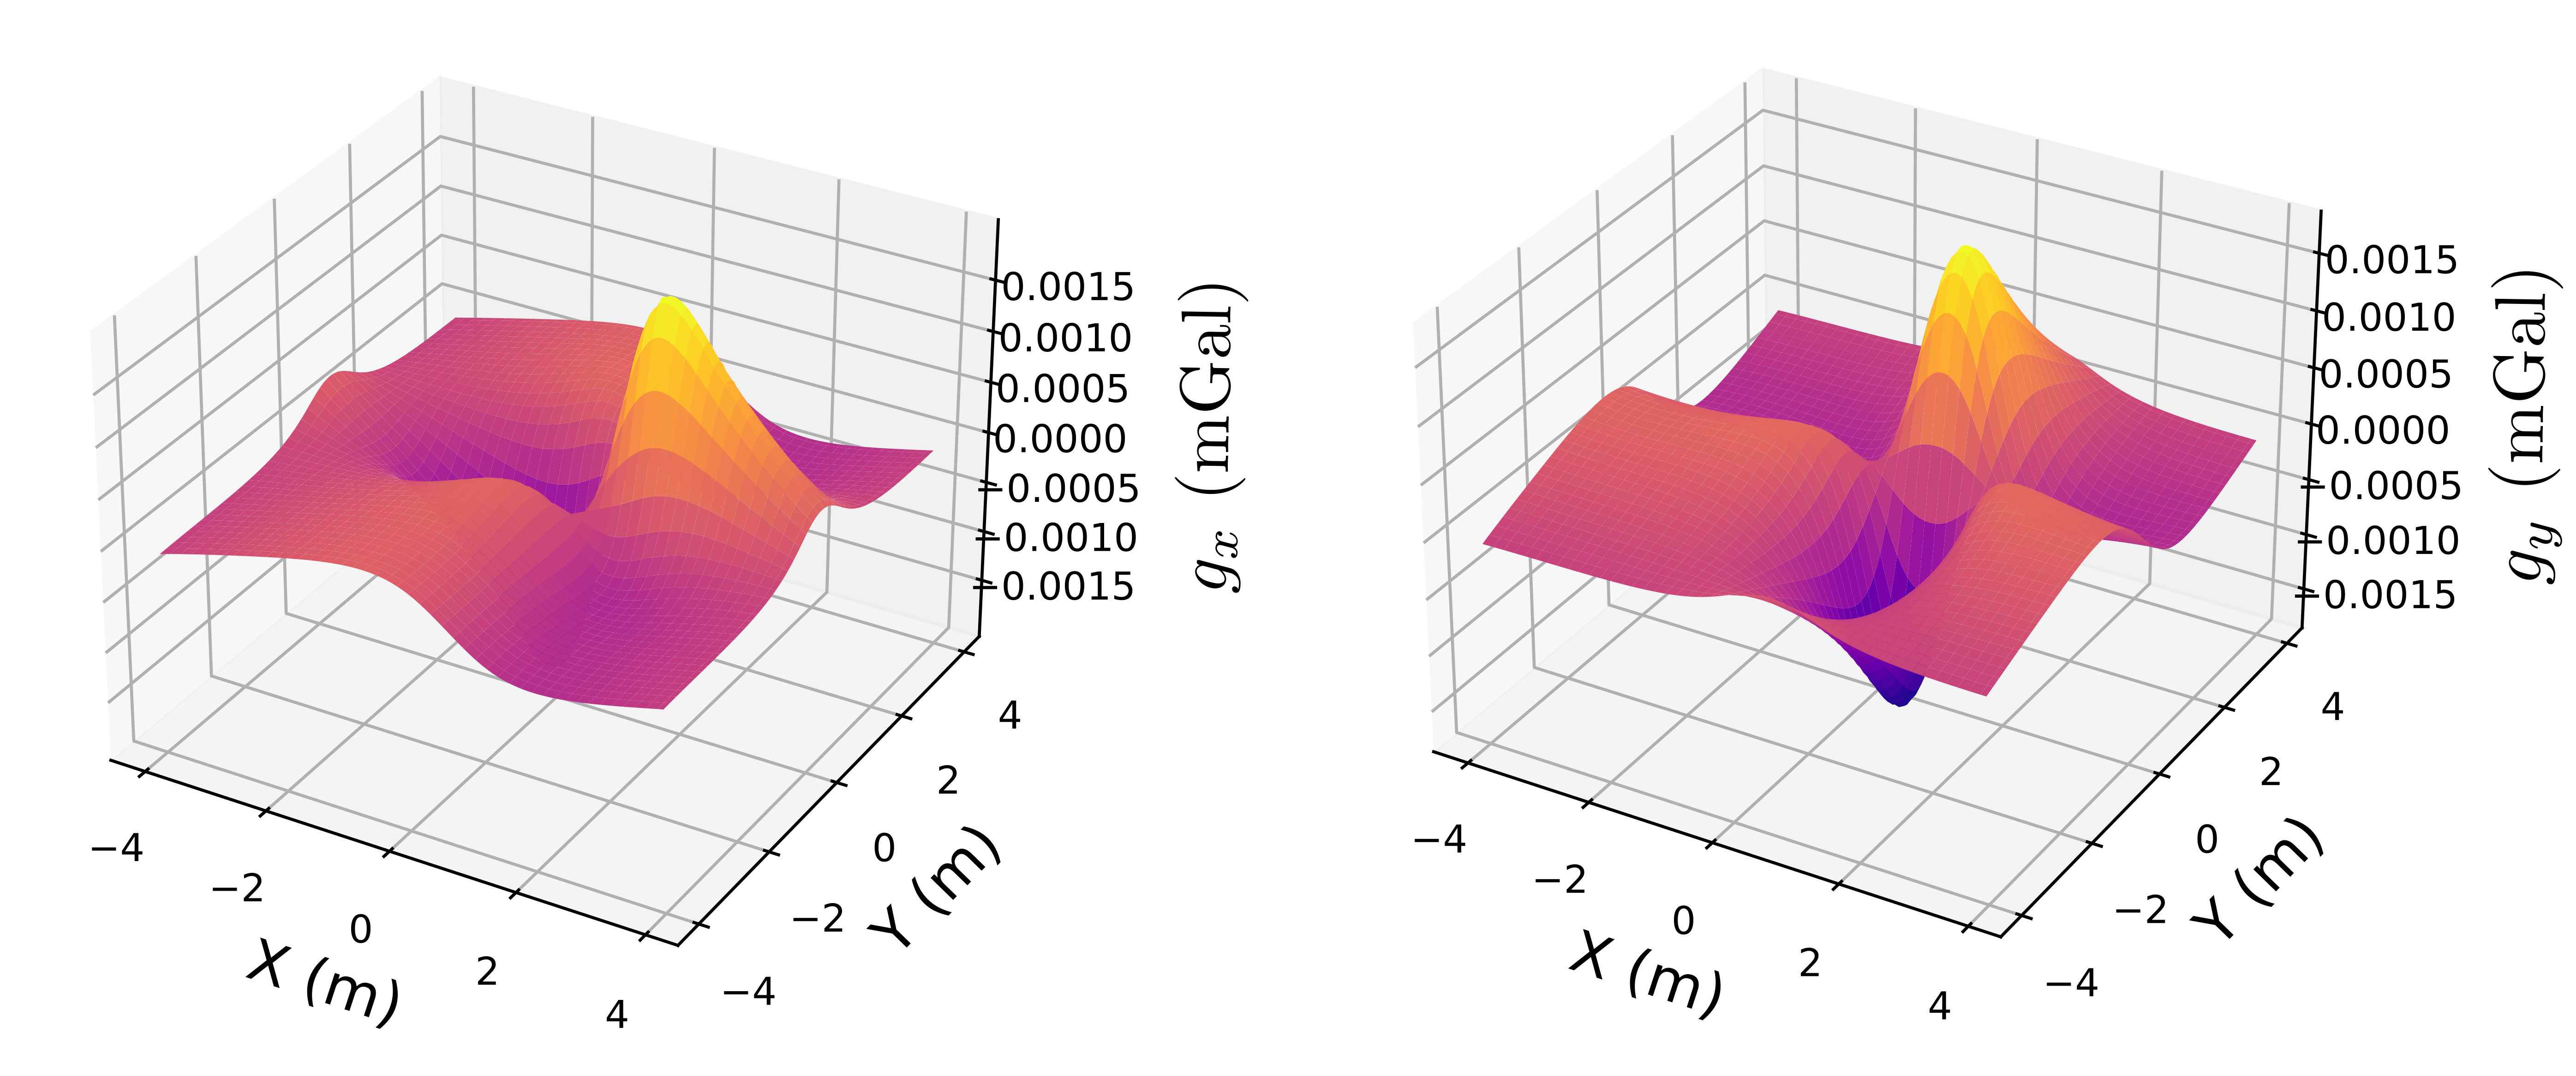
\includegraphics[scale= 0.65]{plots/mass_anomaly_g_x_y.png}
    \caption{Calculation of the $g_{x}$ and $g_{y}$ from Fourier Model.}
\end{figure}

\begin{equation} \label{8}
g_{z} \leftrightarrow G_{z} 
\end{equation}


\noindent Gravity gradient tensor components are the double derivative of the gravitational potential. Equation(\ref{9}) represents the Inverse FFT of multiplication of the matrix of wave vector with Fourier transform of gravity along $z-$ direction. Using this equation(\ref{9}), we can define the full gravity gradient tensor components in ${k_{x}, k_{y}}$ plane. If \textbf{$\Gamma_{i},_{j}$} refers the gravity gradient tensor in $k_{x},k_{y}$ plane then,

\begin{equation} \label{9}
\textbf{$\Gamma_i,_j$}= \mathcal{F}^{-1} \{[K\textbf{(k)}] G_z\textbf{(k)}\} 
\end{equation}

$\because$

\begin{equation}\label{eq_cal3_2}
 {[K\textbf{(k)}]}
=\begin{vmatrix}
\frac{-k_x^2}{|\textbf{k}|} & \frac{-k_x k_y }{|\textbf{k}|} & -i k_x \\
\frac{-k_x k_y}{|\textbf{k}|} & \frac{-k_y^2}{|\textbf{k}|} & -i k_y\\
-i k_y & - i k_y  & {|\textbf{k}|}\\
\end{vmatrix}
\end{equation}


\noindent where $|\textbf{k}| \neq 0 $ , $i,j = x,y,z$ and  $\mathcal{F}^{-1}$ represent the operation of inverse Fourier transform. The matrix form of the whole gravity gradient tensor is given in equation (\ref{tensor_ggt})

\begin{equation} \label{tensor_ggt}
\textbf{$\Gamma_i,_j$}=\begin{vmatrix} %matrix used for determinants
T_{xx} & T_{xy} & T_{xz} \\
T_{yx} & T_{yy} & T_{yz} \\
T_{zx } & T_{zy }& T_{zz}
\end{vmatrix}
\end{equation}    

\noindent Thus, from equations(\ref{8}) and (\ref{9}), it is evident that the complete gravity gradient tensor components may be calculated from the theory of only the vertical component of gravity $(g_{z})$.

\begin{figure*}
    \centering
    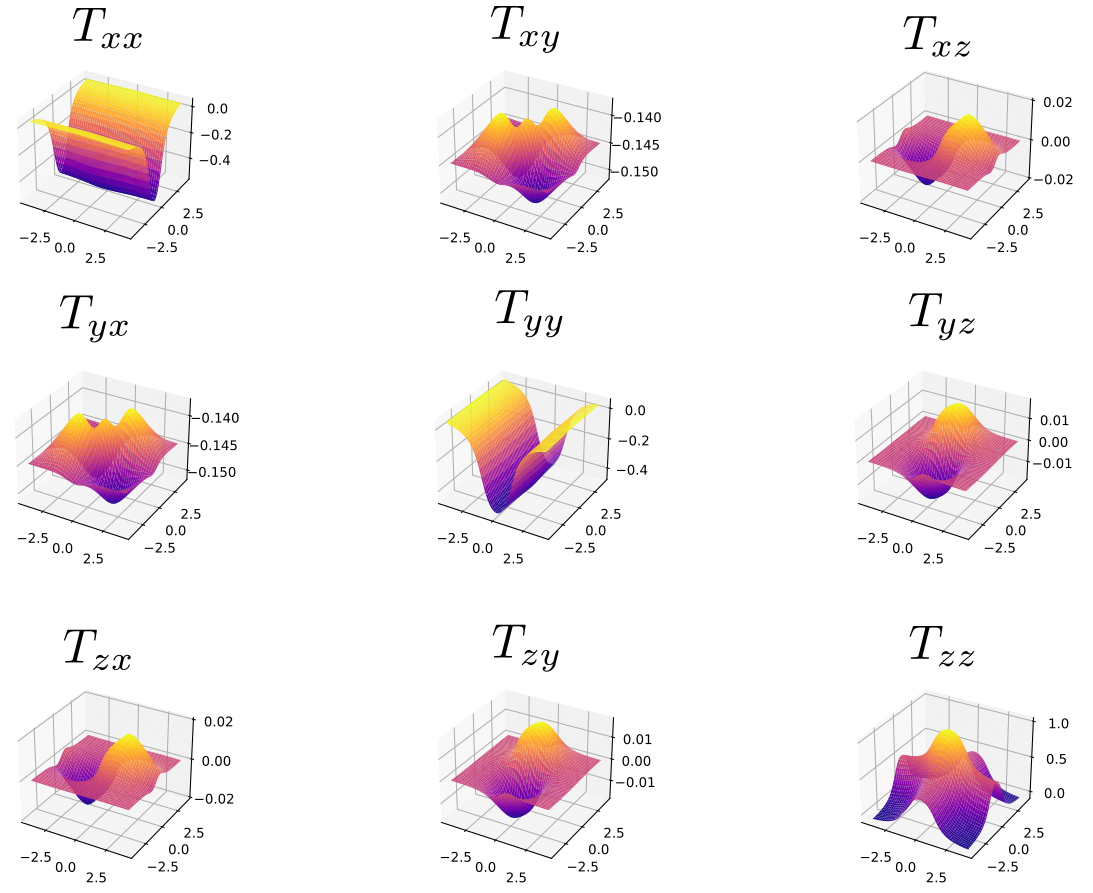
\includegraphics[scale=2.5]{plots/GGT.png}
    \caption
    The FFT derived nine gravity gradient tensor components computed using the vertical
gravity anomaly values from the rectangular prism model.}
\end{figure*}

\subsection{Inverse Modelling}

 This model requires  Gravity Gradient tensor components to calculate the mass of the sub-surface object. The mass formula combines gravitational anomaly and the vertical and horizontal gravity gradient components. The formula is \cite{tang2017analytical},

\begin{equation}\label{mass}
 M=\frac{4({g_x}^2+{g_y}^2+{g_z}^2)^\frac{3}{2}}{T_{xx}+T_{yy}-\sqrt{(T_{xx}-T_{yy})^2+4T_{xy}^2}}
\end{equation}

\begin{figure}[H]
    \centering
    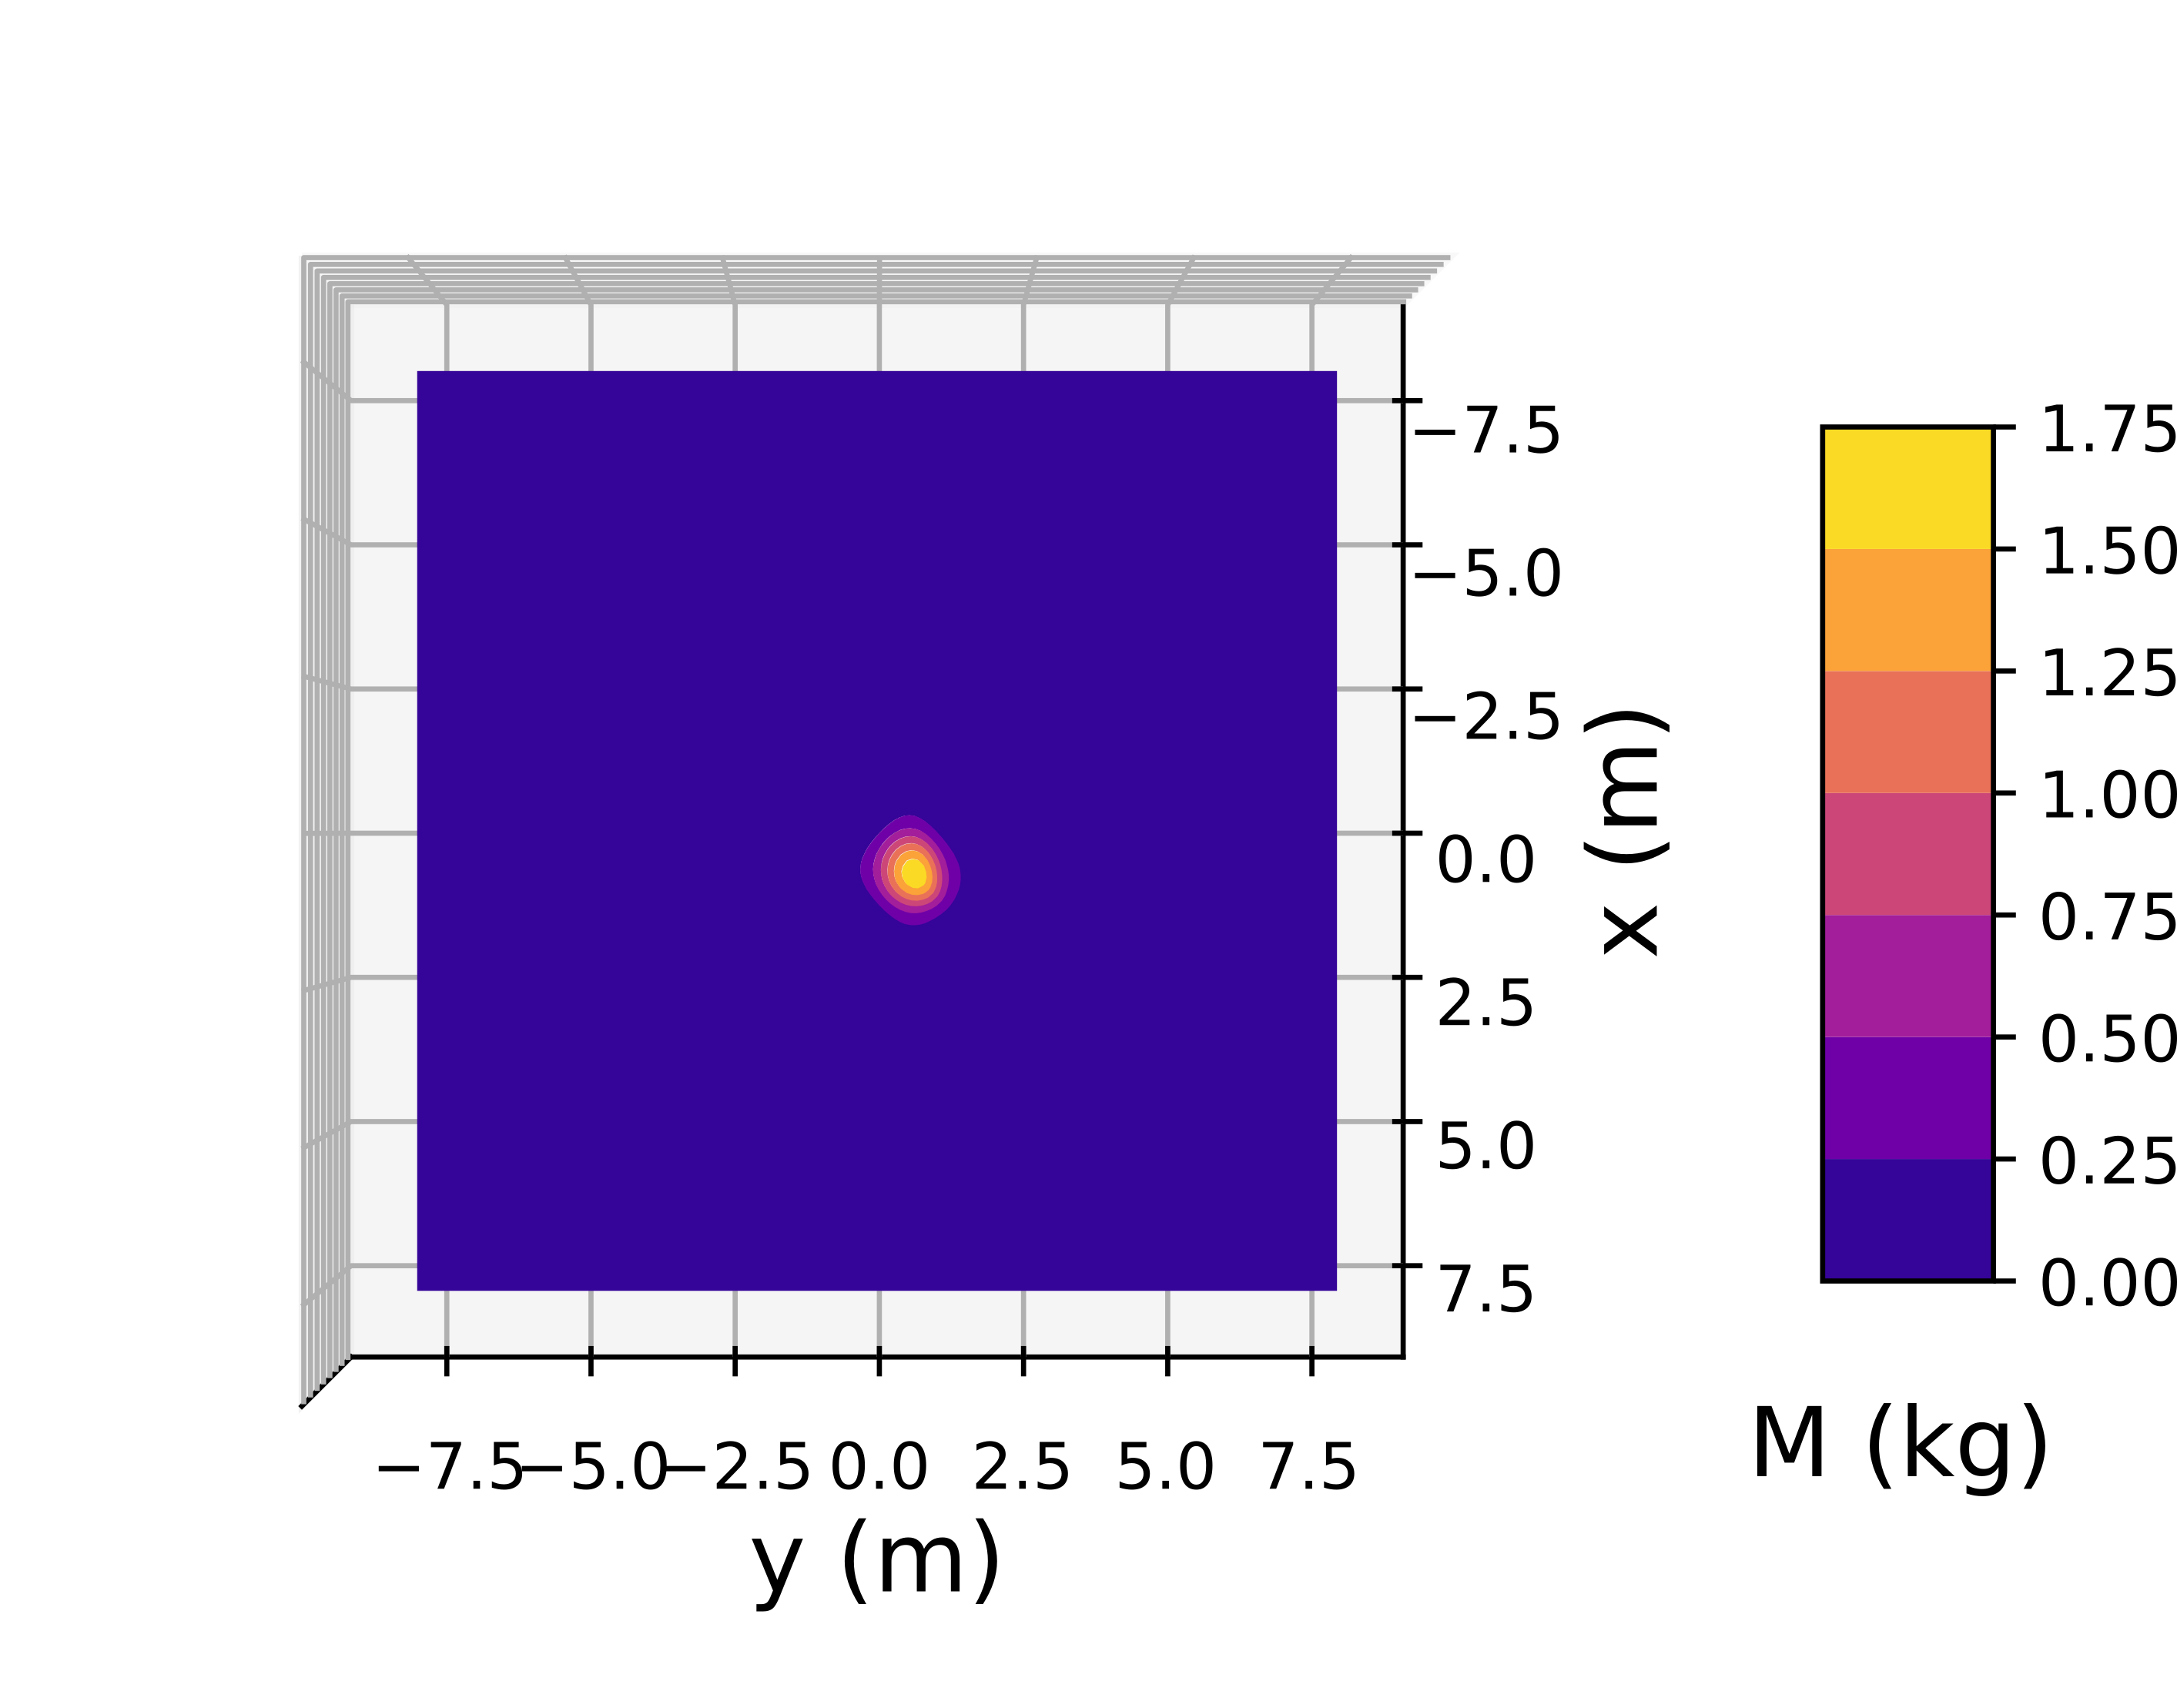
\includegraphics[scale=0.8]{plots/mass_anomaly.png}
    \caption{Detected Mass Anomaly at 1 m depth from base, 330.65 Kg with an estimated center of Mass at (x, y) (0.7000, 0.5260) }
\end{figure}

\section{Result and Discussion}

Using equation (\ref{mass}) is used to calculate the expected mass of the anomaly at different depths {(TABLE-I)}. Similarly, with the help of equation(\ref{mass}), an estimate of the expected mass of different density rocks (TABLE-II) and materials is made in TABLE-III. 
Although estimates are not very accurate, this gives us an idea of the present body, and this could be helpful for archaeologists trying to figure out the best position to dig without disturbing any artifact. This model can also provide a good starting point for any such explorations.\\

\begin{table}[h]
\centering
\caption{Variation of mass with density}
\vspace{.2cm}
\begin{tabular}{|c|c|c|c|c|c|c|}
\hline
\multirow{2}{*}{Object name\vspace{.3cm}}&\multirow{2}{*}{Density\vspace{.5cm}}&\multicolumn{5}{|c|}{Expected Mass(kg)}\\ 
\cline{3-7}
&\small{(kg/m$^{3}$)}&Depth:10m & Depth:20m & Depth: 30m&Depth: 40m&Depth: 50m \\
 \hline
 Gold & 19300&20.19641 & 6.286 & 2.9796 & 1.7174 & 1.1116 \\
 \hline
Silver &10800 & 11.30161 & 3.51796 &1.6673 & 0.96104 & 0.6220 \\
 \hline
  Mild Steel & 7850 &8.21460 & 2.5570 & 1.2119 & 0.6985 & 0.4521 \\
 \hline
 Diamond & 3520 &3.68349 & 1.1465 & 0.5434 & 0.3132  & 0.2027 \\
\hline
Basalt & 2850 &2.98237 & 0.9283& 0.4399 & 0.2536 &0.1641 \\
 \hline
 Marble & 2650 & 2.77308 & 0.8632 & 0.40912 & 0.2358 & 0.1526 \\
 \hline
 Granite & 2450 & 2.56379 & 0.7980 & 0.37824 & 0.218014 & 0.1411\\
 \hline
 Ballast & 1720 & 1.79988 & 0.5602 &0.26554& 0.15305 & 0.09907  \\
 \hline
\end{tabular}
\label{tpl}
\end{table}

\begin{figure}
    \centering
     \caption{Estimated mass of the object for different densities}
      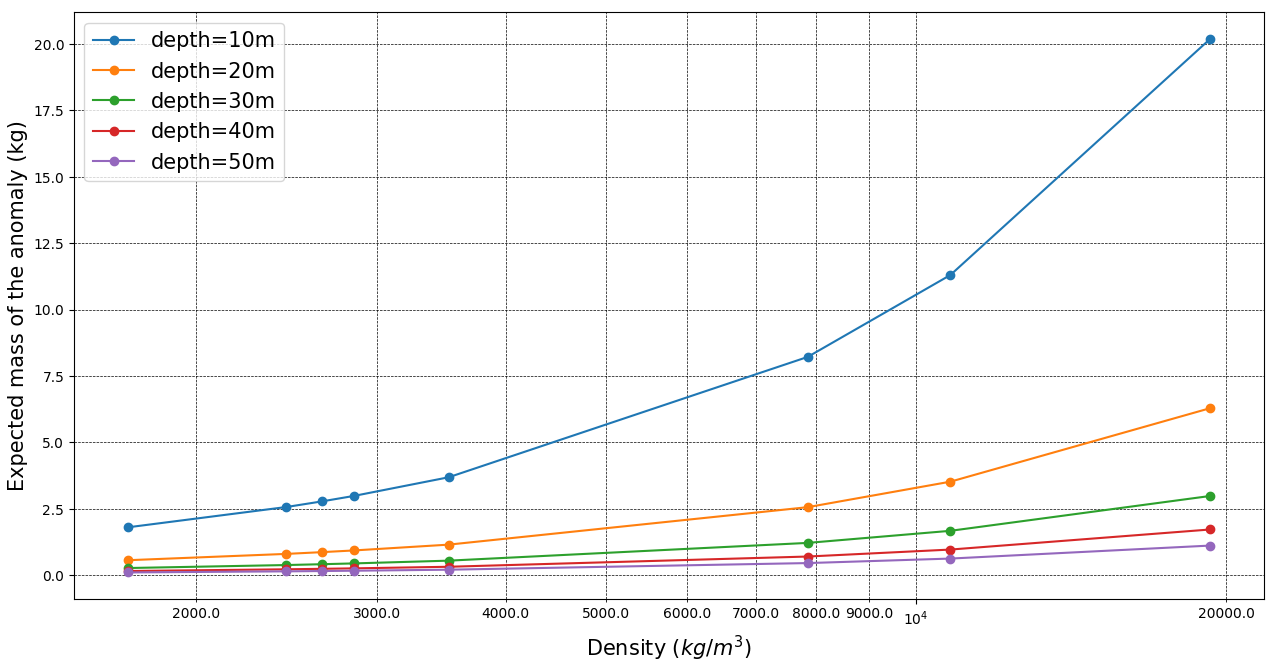
\includegraphics [scale=.5] {plots/depth(10-50).png }
    \label{T_r}
\end{figure}






\newpage
\bibliography{refer}
\bibliographystyle{unsrt}



\end{document}
